\documentclass{beamer}

\usepackage[english]{babel}

\usepackage{appendixnumberbeamer}
\expandafter\def\expandafter\insertshorttitle\expandafter{%
  \insertshorttitle\hfill\insertframenumber\,/\,\inserttotalframenumber}
  
\usepackage{amsmath,amssymb,latexsym,amscd}
\usepackage{amsmath,amsfonts,amsthm} % Math packages
\usepackage{graphicx}
\usepackage{xcolor}
\usepackage{float} 			% para forzar a que las imagenes se queden en un lugar
\usepackage{enumerate}
\usepackage{amsthm}
\usepackage{array}
\usepackage{epstopdf}
\usepackage{ragged2e}		% para justificar
\usepackage{etoolbox}
\usepackage{multirow}
\usepackage{bibentry}
\usepackage{array}

\justifying

\theoremstyle{plain}

\apptocmd{\frame}{}{\justifying}{}
\apptocmd{\itemize}{}{\justifying}{}

\newcommand{\linea}{\noindent\makebox[\linewidth]{\rule{\textwidth}{1pt}}}

\newtheorem{thm}{Theorem}
\newtheorem{obj0}[thm]{Objetivo [v0]}
\newtheorem{obj1}[thm]{Objetivo [v1]}
\newtheorem{obj2}[thm]{Objetivo [v2]}
\newtheorem{simp}[thm]{Posibles simplificaciones}

\numberwithin{equation}{section} % Number equations within sections (i.e. 1.1, 1.2, 2.1, 2.2 instead of 1, 2, 3, 4)
\numberwithin{figure}{section} % Number figures within sections (i.e. 1.1, 1.2, 2.1, 2.2 instead of 1, 2, 3, 4)
\numberwithin{table}{section} % Number tables within sections (i.e. 1.1, 1.2, 2.1, 2.2 instead of 1, 2, 3, 4)

%\usetheme{Montpellier}
%\usetheme{Madrid}
%\usetheme{Marburg}
\usetheme{CambridgeUS}

\usecolortheme{whale}

\setbeamercolor{frametitle}{bg=gray,fg=white}
\setbeamertemplate{blocks}[rounded][shadow=false]
\setbeamercolor{block title}{use=structure,fg=black,bg=gray!15!white}
\setbeamercolor{block body}{use=structure,fg=black,bg=gray!5!white}

\input{macros.tex}

\begin{document}

%\renewcommand{\inserttotalframenumber}{\pageref{lastslide}}

\title[]{Classification of Musical Periods}
\author[Mauricio Toledo-Acosta]{Gerardo Mauricio Toledo Acosta\\
\medskip
{\small Postdoctorado\\ 
Laboratorio de Semántica Computacional\\
Centro de Investigación en Ciencias\\
UAEM
} 
}

\date{\today}

{\usebackgroundtemplate{
\includegraphics[width=\paperwidth]{BackgroundPS2.png}}
\maketitle }

%=====================================================================================



{
\usebackgroundtemplate{
\includegraphics[width=\paperwidth]{BackgroundPS2.png}}

\begin{frame}
\frametitle{Objetivo}

\uncover<1->{En la historia de la m\'usica hay varios periodos muy diferentes:}

\uncover<2->{
\begin{itemize}
\item Periodo barroco: 1600-1750.
\item Periodo cl\'asico: 1750-1820.
\item Periodo rom\'antico: 1820-1900.
\end{itemize}}

\uncover<3->{
\begin{obj0}
\justifying
?`Es posible clasificar la m\'usica en estos periodos usando una red neuronal?
\end{obj0}
}

\uncover<4->{
\begin{obj1}
\justifying
?`Es posible clasificar representaciones gr\'aficas de la m\'usica en estos periodos usando una red neuronal?
\end{obj1}
}

\end{frame}

%----------------------------------------


\begin{frame}
\frametitle{2. ?`C\'omo abordar el problema?}
\justifying

\begin{table}[h!]

\begin{center}
\begin{tabular}{p{0.45\textwidth} | p{0.45\textwidth}}
\justifying
\uncover<1->{
Tengo un dataset de 1549 
archivos midi de piezas de piano de los tres periodos.} &

\uncover<2->{
Origen: Kaggle, The MAESTRO Dataset (Tensorflow), websites de midis.} 
\end{tabular}
\end{center}
\end{table}


\uncover<3->{
He generado un piano-roll de cada archivo midi:

\begin{table}[h!]
\begin{center}
\begin{tabular}{ccc}

Barroco & Cl\'asico & Rom\'antico \\

\begin{minipage}{.3\textwidth}
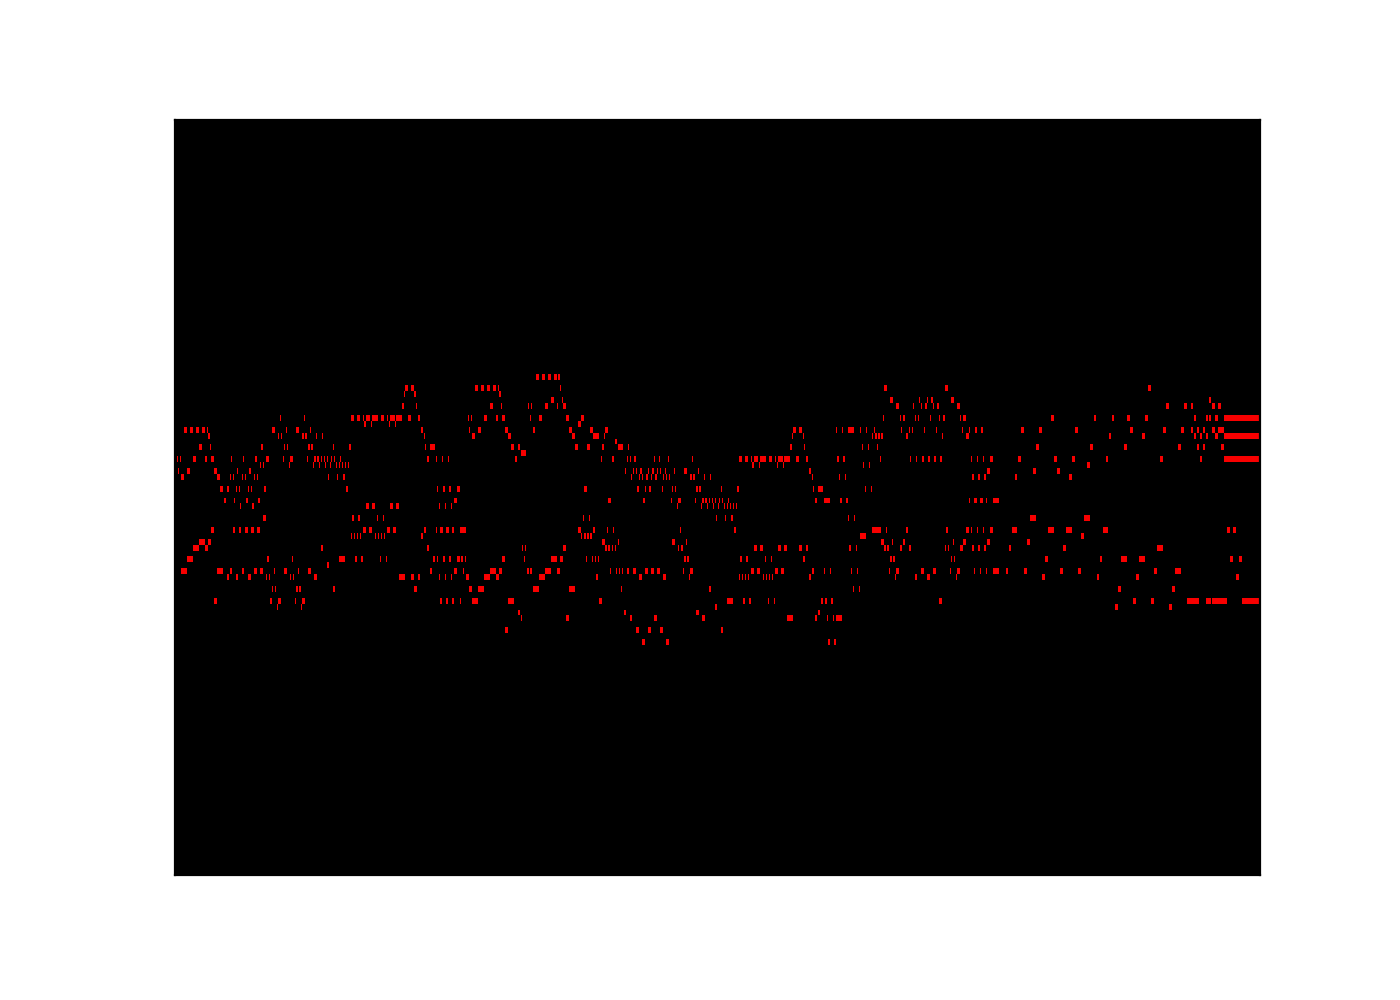
\includegraphics[width=\linewidth, height=25mm]{1barrocoA.png}
\end{minipage}

 &
\begin{minipage}{.3\textwidth}
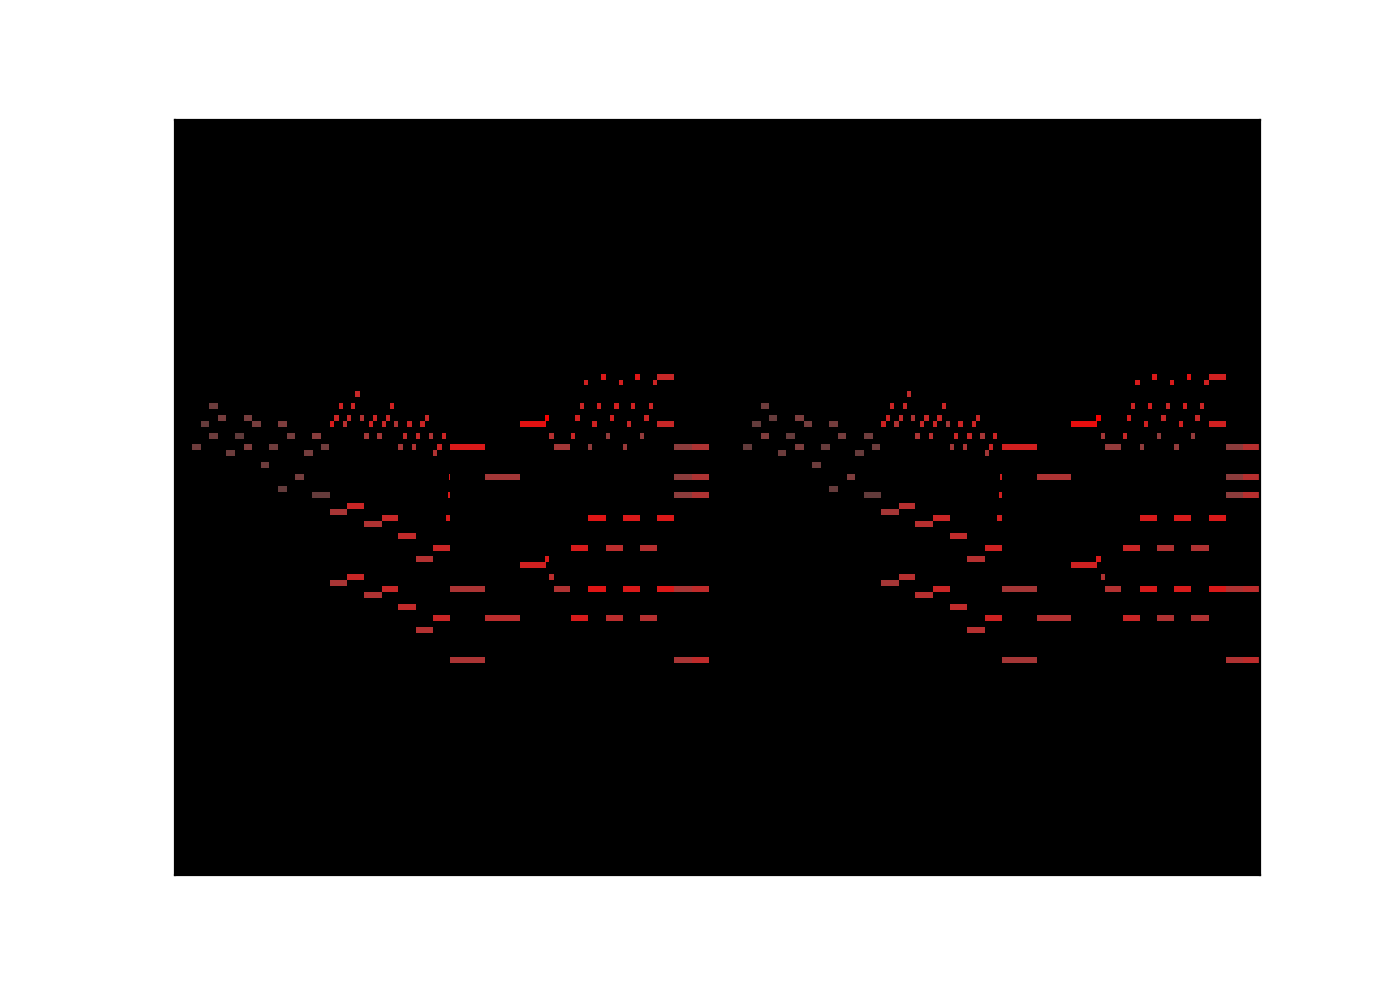
\includegraphics[width=\linewidth, height=25mm]{2clasicoA.png}
\end{minipage}

&

\begin{minipage}{.3\textwidth}
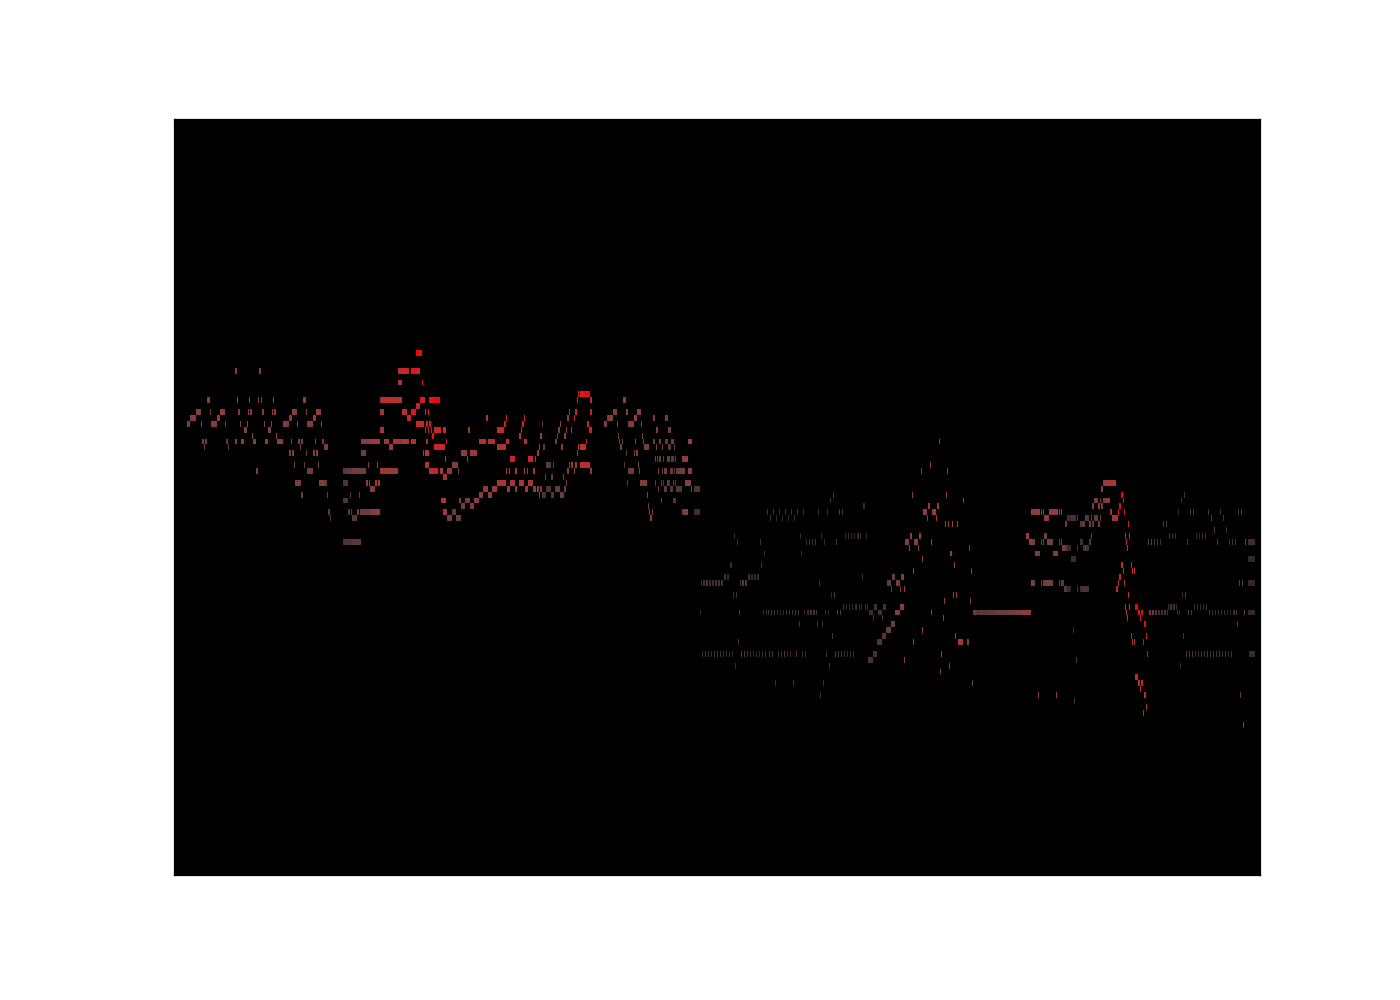
\includegraphics[width=\linewidth, height=25mm]{3romanticoA.png}
\end{minipage}


\\
\end{tabular}
\end{center}
\end{table}

}


\uncover<4->{
\begin{obj2}
Entrenar una red neuronal para clasificar las imagenes.
\end{obj2}
}
\end{frame}

%----------------------------------------


\begin{frame}
\frametitle{Posibles dificultades derivadas del dataset}
\justifying

\begin{itemize}[<+->]
\item No son tantas instancias, 1893.

\item Tama\~nos relativos desproporcionados
\begin{figure}[H]
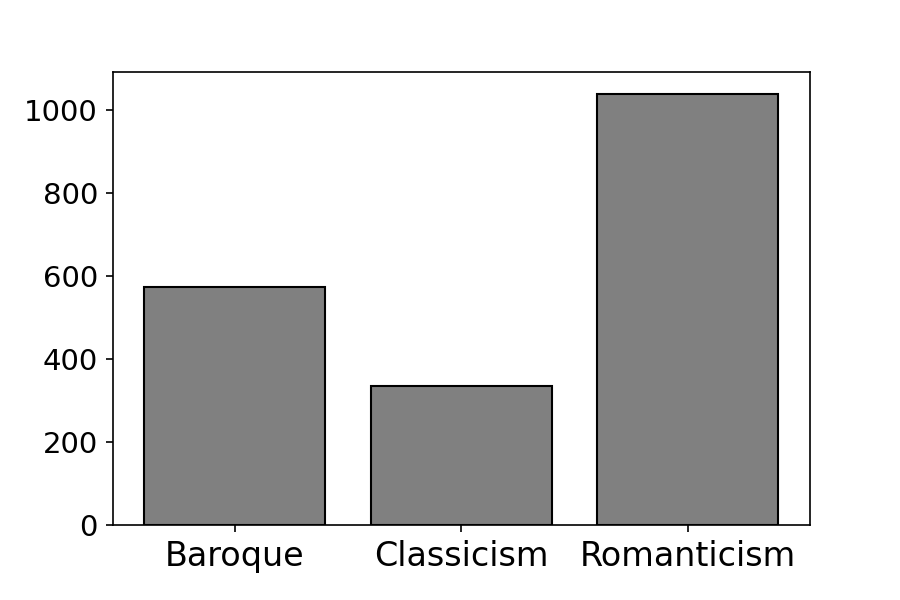
\includegraphics[height=27mm]{histogram_periods.png}
\end{figure}


\item Configuraci\'on correcta de los par\'ametros de las imagenes.

\end{itemize}

\end{frame}

%----------------------------------------

\begin{frame}
\frametitle{Primeros resultados}
\justifying

\begin{table}[h!]
\begin{center}
\begin{tabular}{ccc}

\begin{minipage}{.3\textwidth}
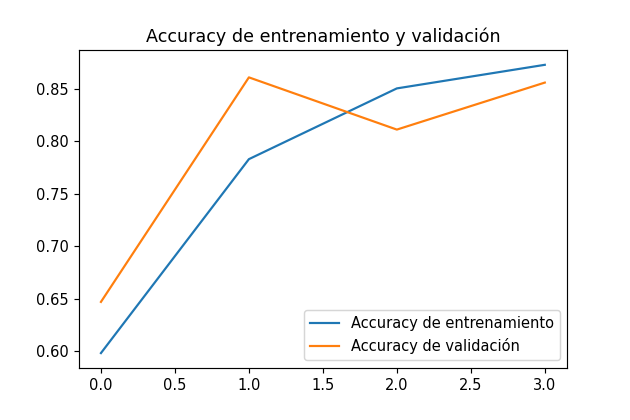
\includegraphics[width=\linewidth, height=25mm]{02-TA.png}
\end{minipage}

 &
\begin{minipage}{.3\textwidth}
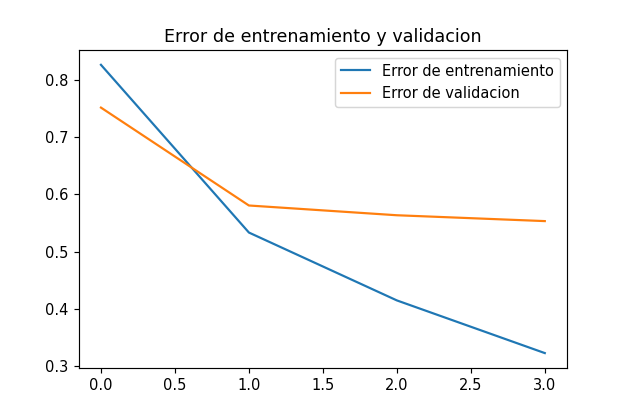
\includegraphics[width=\linewidth, height=25mm]{02-TE.png}
\end{minipage}

&

\begin{minipage}{.3\textwidth}
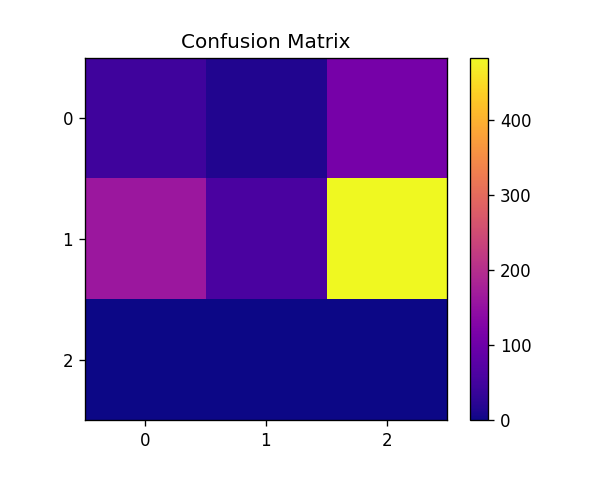
\includegraphics[width=\linewidth, height=25mm]{02-CM.png}
\end{minipage}
\\
\end{tabular}
\end{center}
\end{table}

Hay muy pocas instancias de entrenamiento.

\end{frame}

%----------------------------------------

\begin{frame}
\frametitle{PCA sobre las features}

\begin{itemize}
\justifying
\item Cada archivo MIDI tiene asociado un tensor Canales$\times$Rango$\times$Duraci\'on, se suma sobre el primer eje para tener una matriz Rango$\times$Duraci\'on, la aplanamos:

\begin{figure}[H]
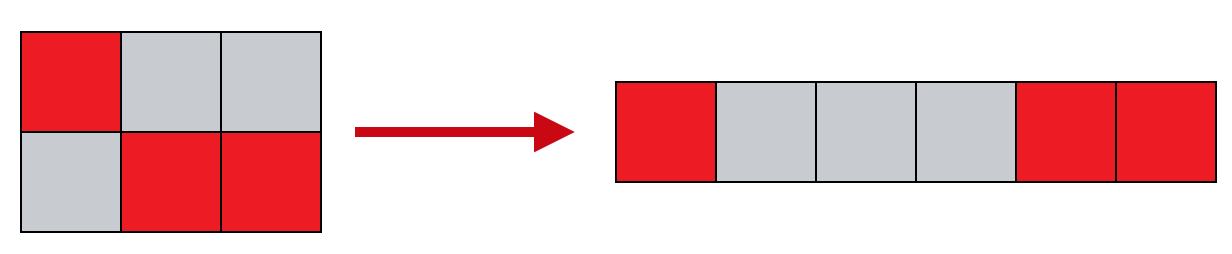
\includegraphics[height=5mm]{Flatten.png}
\end{figure}

\item Formamos una matriz donde cada rengl\'on es un archivo MIDI aplanado. Tiene forma 1893$\times$29965936. Aproximadamente, s\'olo el 2$\%$ son datos. 

\medskip

\item Debido al tama\~no de la matriz, se usan matrices \texttt{sparse} de \texttt{scipy}. En lugar de PCA, usamos \texttt{truncatedSVD}.
\medskip

\end{itemize}

\end{frame}

%----------------------------------------

\begin{frame}
\frametitle{PCA sobre las features}


\begin{itemize}
\justifying
\item S\'olo pude calcular 6 componentes.


\begin{table}[h!]
\begin{center}
\begin{tabular}{cc}

\begin{minipage}{.4\textwidth}
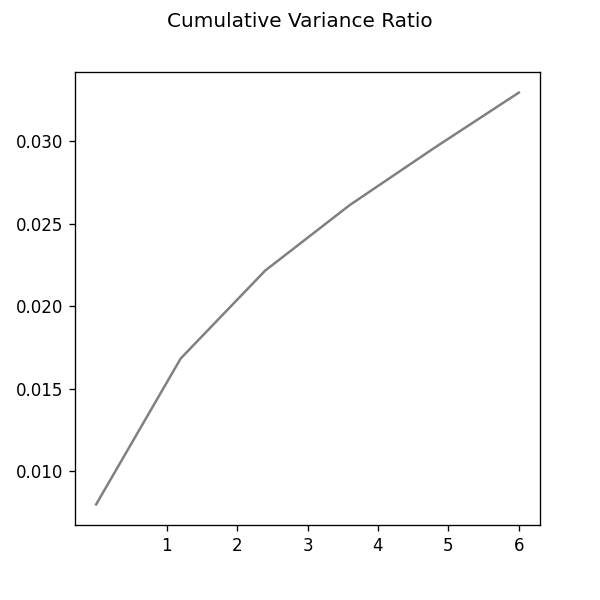
\includegraphics[width=\linewidth, height=40mm]{PCA-6D.png}
\end{minipage}

 &
\begin{minipage}{.4\textwidth}
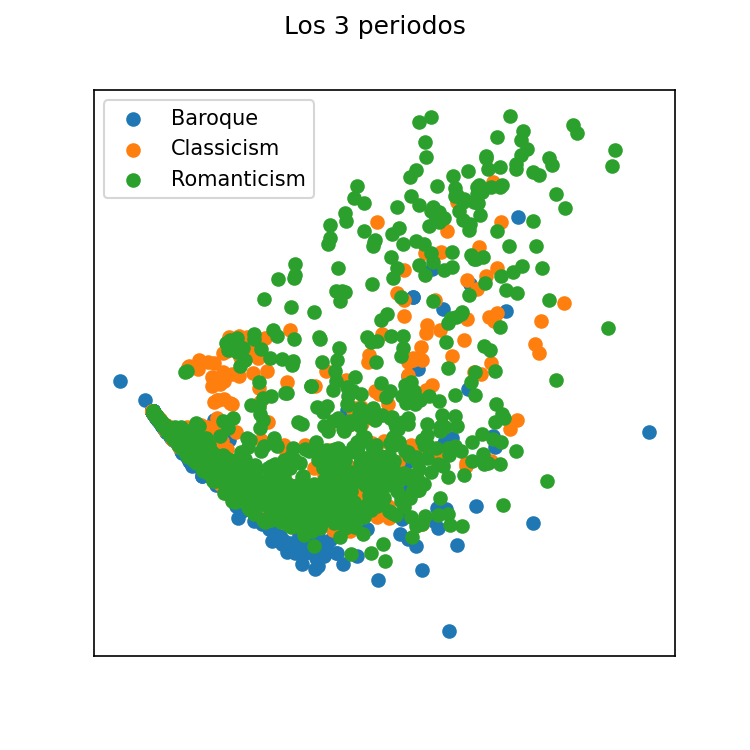
\includegraphics[width=\linewidth, height=40mm]{PCA.png}
\end{minipage}
\\
\end{tabular}
\end{center}
\end{table}

\item Alternativas: Latent Dirichlet Allocation (LDA), \texttt{MiniBatchSparsePCA}.

\item Falta aplicar regresi\'on logistica o alg\'un otro m\'etodo de clasificaci\'on.

\end{itemize}

\end{frame}
}

%----------------------------------------

\begin{frame}
\frametitle{PCA sobre las features}


\begin{itemize}
\justifying

\item Podr\'ia reducirse el tamaño de las matrices en el segundo eje:

\begin{figure}[H]
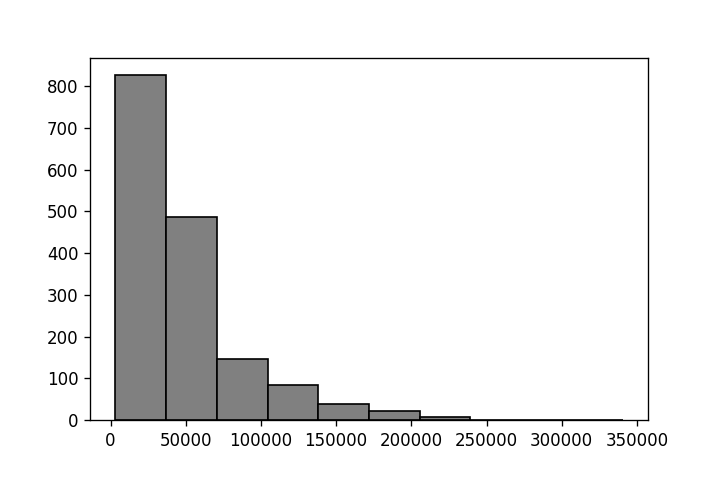
\includegraphics[height=30mm]{Histograma-duraciones.png}
\end{figure}

\item El segundo eje del tensor se redujo lo m\'as posible:

\begin{figure}[H]
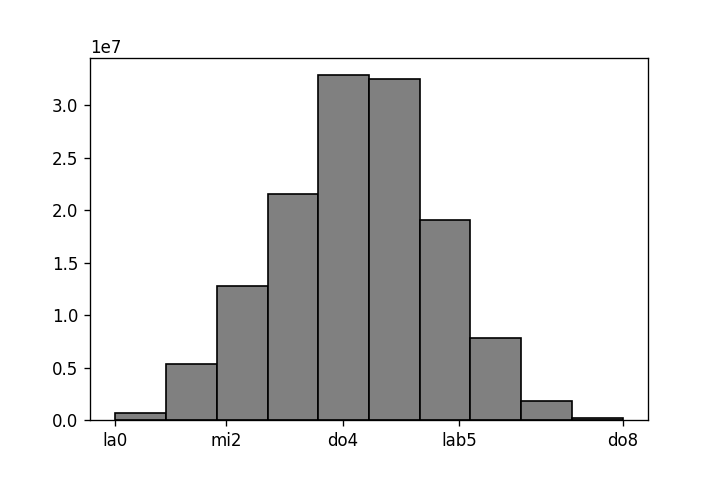
\includegraphics[height=30mm]{Histograma-notas.png}
\end{figure}

\end{itemize}

\end{frame}

%----------------------------------------

\begin{frame}
\frametitle{Aumento de instancias}

\begin{itemize}
\justifying 

\item Transposiciones: Tocar la misma pieza un poco m\'as agudo o grave. Con esto, consegu\'i 4 veces m\'as instancias.

\begin{table}[h!]
\begin{center}
\begin{tabular}{cc}

\begin{minipage}{.4\textwidth}
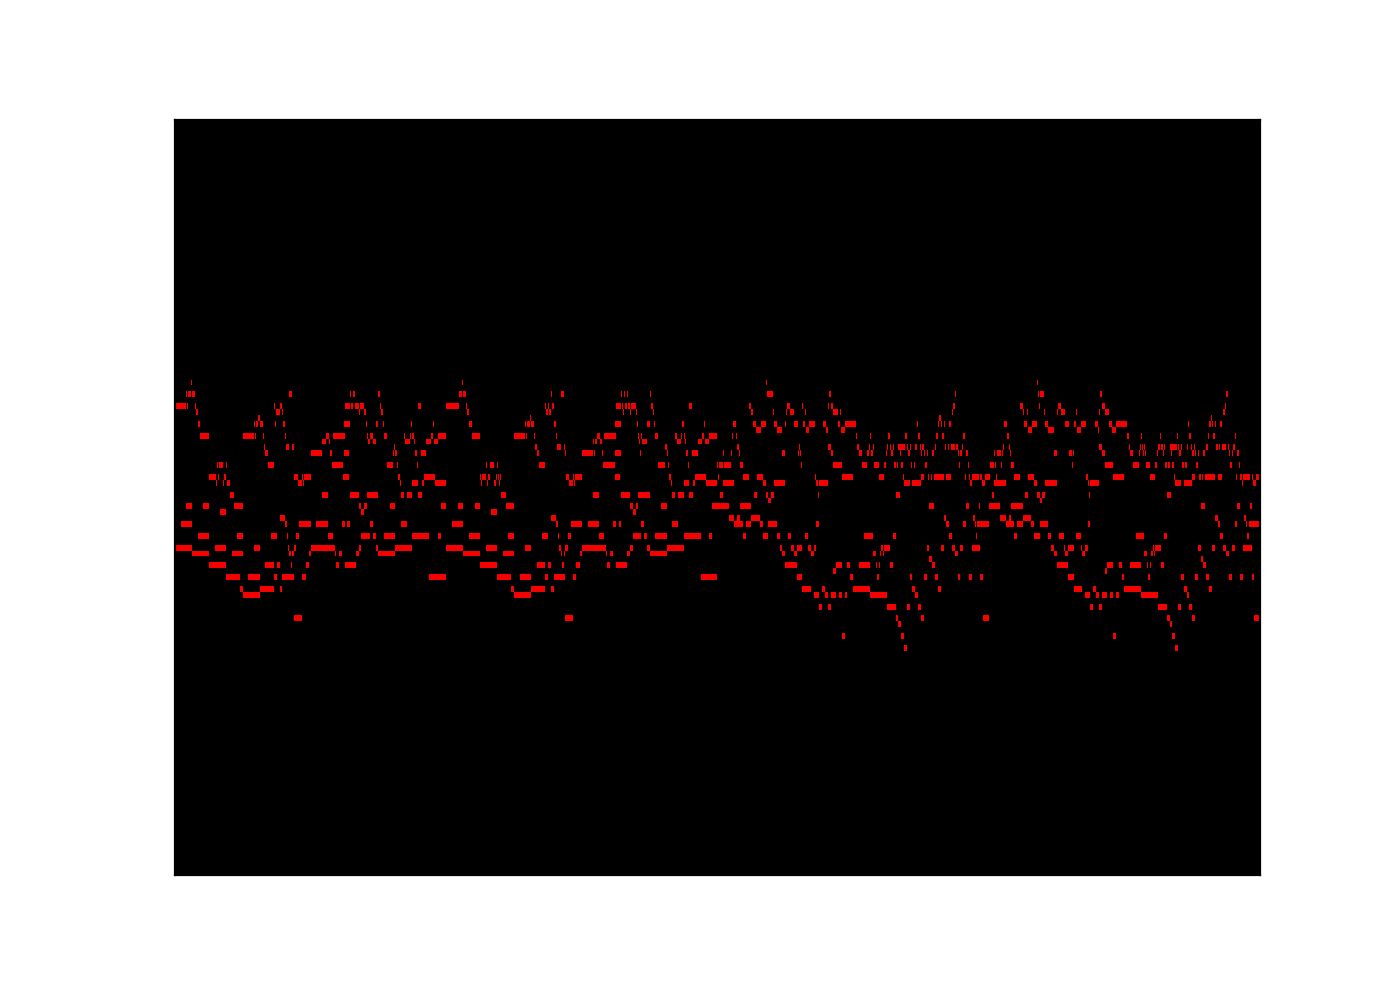
\includegraphics[width=\linewidth, height=40mm]{T-root.png}
\end{minipage}

 &
\begin{minipage}{.4\textwidth}
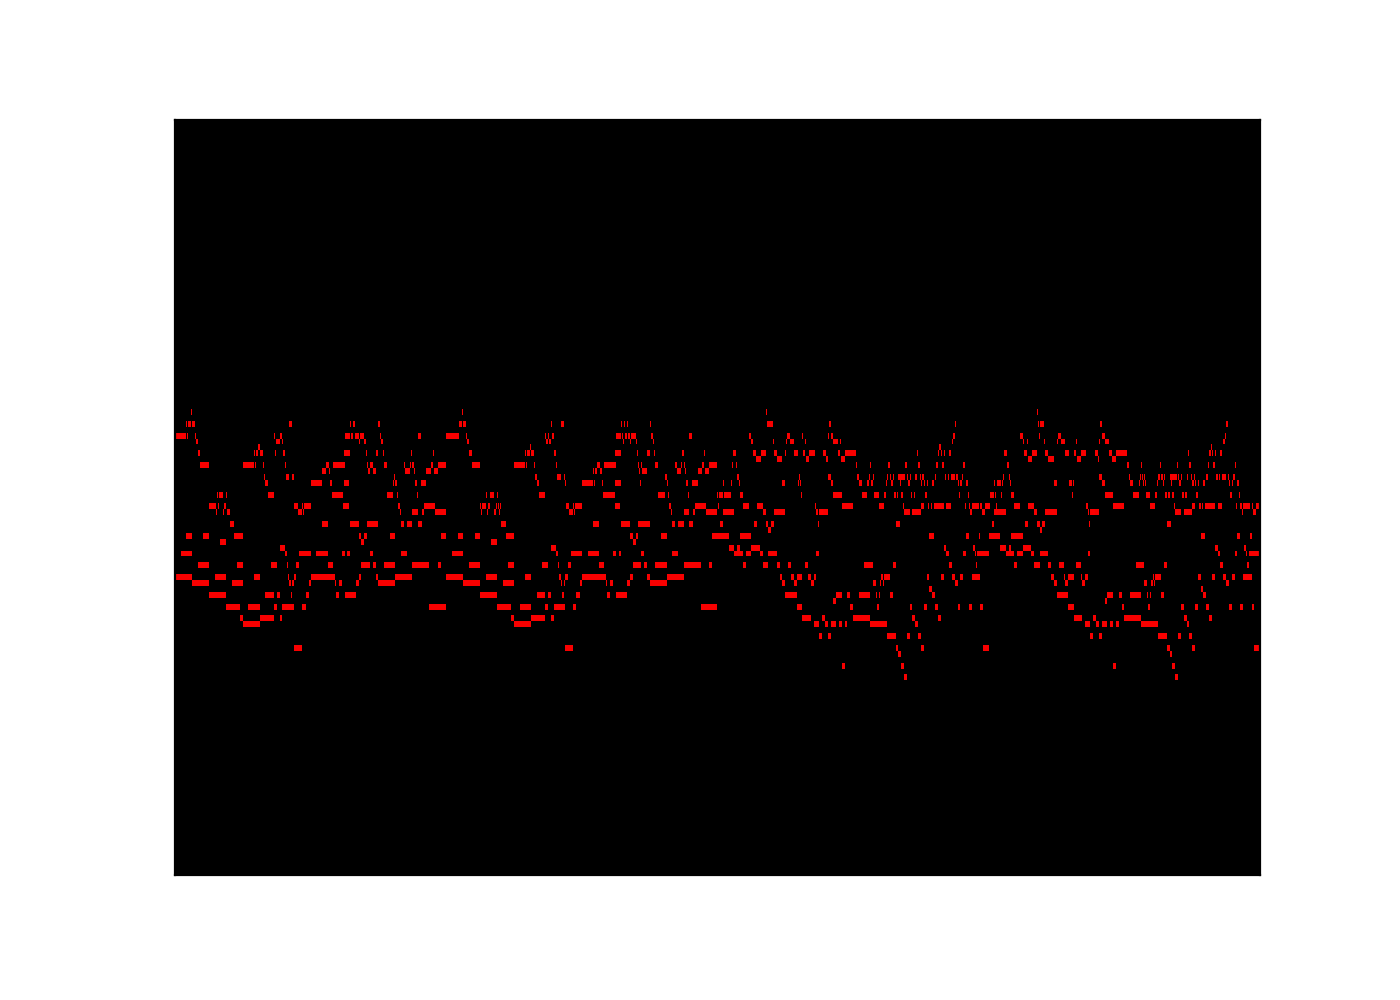
\includegraphics[width=\linewidth, height=40mm]{T-5d.png}
\end{minipage}
\\
\end{tabular}
\end{center}
\end{table}

\item Puede haber otras opciones para alterar las im\'agenes de una \emph{buena} manera (simetr\'ias, re-arreglos).

\end{itemize}

\end{frame}

%----------------------------------------

\begin{frame}
\frametitle{Nuevos resultados}


\end{frame}

%----------------------------------------

\end{document}